\section{HERRAMIENTAS Y ENTORNO DE DESARROLLO}

El desarrollo, instrumentación y despliegue del sistema se fundamenta en un ecosistema tecnológico moderno, combinando herramientas de automatización de navegador, infraestructura serverless en la nube y entornos de procesamiento de lenguaje natural. En la Tabla~\ref{tab:stack_tecnologico} se sintetizan los componentes principales del stack técnico.

\begin{table}[htbp]
    \centering
    \small
    \caption{Stack Tecnológico, Herramientas de Desarrollo y Versiones del Sistema}
    \label{tab:stack_tecnologico}
    \begin{tabularx}{\linewidth}{>{\raggedright\arraybackslash}p{3.8cm} >{\raggedright\arraybackslash}p{4.4cm} L}
        \toprule
        \textbf{Capa Arquitectónica} & \textbf{Tecnología / Versión} & \textbf{Función y Rol Específico en el Ecosistema} \\
        \midrule
        Entorno de Ejecución & Node.js v24.11 LTS & Motor de ejecución asíncrono para scrapers, pipelines de ingesta y scripts de sincronización. \\
        Lenguaje de Tipado & TypeScript 5.x & Definición de interfaces estáticas para modelos de datos (\nolinkurl{CanastaItem}, \nolinkurl{MedicamentoItem}). \\
        Automatización Web & Playwright 1.48 & Control de Chromium vía CDP, resolución de scroll infinito y manejo de contextos persistentes. \\
        Base de Datos Principal & Neon Serverless PostgreSQL & Motor relacional con escalamiento automático, particionamiento declarativo mensual y triggers PL/pgSQL. \\
        Indexación Vectorial & Extensión \nolinkurl{pgvector} & Almacenamiento e indexación HNSW para vectores de 1024 dimensiones con métrica de distancia coseno. \\
        Almacenamiento de Objetos & Neon Object Storage S3 & Bucket \nolinkurl{assets} compatible con AWS S3 para persistencia permanente de imágenes de productos. \\
        Inteligencia Artificial & NVIDIA NIM API & Generación de representaciones vectoriales densas para búsqueda semántica híbrida en SICOES. \\
        Plataforma Web Frontend & Next.js 14 (App Router) & Renderizado híbrido (SSR), rutas API REST internas y componentes de visualización reactiva. \\
        Estilos y Cartografía & TailwindCSS y Leaflet & Maquetación adaptable para dispositivos móviles y renderizado de mapas interactivos con capas OpenStreetMap. \\
        Asistente Conversacional & Telegram Bot API & Interfaz móvil accesible con soporte de teclados inline interactivos y captura de logs en tiempo real. \\
        Tipografía y Reporte & MiKTeX 25.4 (pdfTeX) & Sistema tipográfico para la compilación formal del informe académico bajo el estándar APA 7. \\
        \bottomrule
    \end{tabularx}
    \tablenote{Resumen de las tecnologías, frameworks y plataformas integradas en la solución integral de minería web multidimensional.}
\end{table}

\subsection{Telemetría de Consola y Monitoreo de Extracción en Vivo}
Para asegurar la observabilidad operativa y medir con precisión la ejecución de cada fase del pipeline, los crawlers implementan un sistema de telemetría y logging estructurado en tiempo real. Como se evidencia en la Figura~\ref{fig:scraper_telemetria}, la consola expone de forma continua el progreso de recolección:

\begin{itemize}[leftmargin=*]
    \item Confirmación de procesamiento por categoría (\textit{``Extracción completada sin omisiones''}).
    \item Monitoreo de tarjetas DOM analizadas e incremento incremental de productos nuevos por sucursal.
    \item Registro del volumen global acumulado al finalizar el rastreo de tiendas (alcanzando \textbf{17,821 productos} en catálogo de supermercado).
    \item Transición inmediata hacia la fase reactiva de verificación e inserción masiva en lote (\textit{bulk upsert}) sobre la tabla operacional \texttt{canasta\_precios} en Neon Serverless PostgreSQL.
\end{itemize}

\begin{figure}[htbp]
    \centering
    \caption{Registro en Terminal de la Extracción en Vivo e Inserción de 17,821 Productos en Neon}
    \label{fig:scraper_telemetria}
    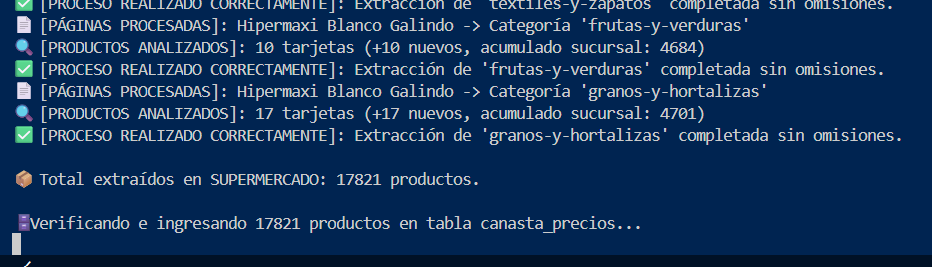
\includegraphics[width=0.95\linewidth]{figuras/terminal_scraper_extraccion_real.png}
    \figurenote{Captura de la ejecución en vivo del agente de extracción \texttt{scraper\_hipermaxi.mjs}. Ilustra el procesamiento exhaustivo de sucursales (p. ej., Blanco Galindo), la consolidación de 17,821 productos y el inicio de la verificación e inserción en base de datos sin errores de omisión.}
\end{figure}

Esta instrumentación permite detectar de forma proactiva degradaciones de rendimiento en las conexiones de red, verificar la concurrencia de inserción en Neon y auditar la integridad de los datos recolectados.
